%
% main.tex -- Paper zum Thema <luke>
%
% (c) 2020 Autor, OST Ostschweizer Fachhochschule
%
% !TEX root = ../../buch.tex
% !TEX encoding = UTF-8
%
\chapter{Oberflächenwasserwellen\label{chapter:luke}}
\kopflinks{Lukes Lagrangian}
\begin{refsection}
\chapterauthor{Sven Schlömmer}

Die Dynamik von Wasserwellen ist ein komplexes Gebiet mit vielen Anwendungen in den Ingenieurwissenschaften und Umweltmodellierung.
Dabei werden in der Regel Modelle von nicht linearen Gleichung nummerisch gelöst.
Jedoch kann durch die Verwendung des Variationsprinzips mathematische Formulierungen entwickelt werden, welche es ermöglichen die Bewegung von Wasserwellen auf elegante Weise zu beschreiben.
Es gibt zwei variationsbasierte Formulierungen für Oberflächenwellen welche häufig Anwendung finden um die Bewegung von Wasserwellen zu modellieren und verstehen.
Das ist der Luke´s Lagrangian von J. C. Luke, sowie das hamiltonische Prinzip von Zakharov.
In diesem Kapitel wird Luke´s Lagrangian verwendet.

Wasserwellen tendieren dazu ihre Energie zu minimieren.
Dies bestätigt die physikalischen Prinzipien der minimalen Energie und Energieerhaltung.
Durch die minimierung der Lagrange-Funktion über das Variationsprinzip, wird die Energie des Systems minimieren und erhaltet ein Gleichungssystem, welche die Konfiguration der Wasserwelle beschreibt.
Dies führt zur Herleitung von Bewegungsgleichungen, welche die Zeitliche Änderung der Wasserwelle definieren.
Somit wird das Variationsprinzip mit der Lagrange-Funktion von Luke angewendet, um die natürliche Tendenz von Wasserwellen zur Energieminimierung mathematisch zu formulieren und daraus physikalisch relevante Gleichungen abzuleiten.

Um dieser vorgang zu demonstrieren wird im Abschnitt \ref{luke:section:Luke_Lagrangian} Luke´s Lagrangian beschrieben und erweitert um mehr Freiheitsgrade zu bekommen.
Nach der Erweiterung des Luke´s Lagrangian wird im Aschnitt \ref{luke:section:SeichtenGewaesser} einen Ansatz für Oberflächenwellen im seichten Gewässer definiert. Dieser wird dann in denn Lagrangian eingefügt und vereinfacht. Über die Variation des Minimalprinzips werden daraufhin die Euler-Lagrange-Gleichungen aufgestellt mit denen Gleichungen für Wasserwellen hergeleitet werden. Jene Gleichungen werden daraufhin mit schon bekannten Gleichungssysteme für Wasserwellen in seichten Gewässer verglichen.

%
% einleitung.tex -- Beispiel-File für die Einleitung
%
% (c) 2020 Prof Dr Andreas Müller, Hochschule Rapperswil
%
% !TEX root = ../../buch.tex
% !TEX encoding = UTF-8
%

\section{Lagrange-Funktion von Luke\label{luke:section:Luke_Lagrangian}}
\kopfrechts{Lagrange-Funktion von Luke}

1967 veröffentlichte J. C. Luke \cite{luke:Luke1967} eine Lagrange-Funktion, mit welcher über ein Variationsprinzip die Bewegungen von Oberflächenwellen auf einer freien Fluidoberfläche unter Einwirkung der Schwerkraft berechnet werden kann.
Genau gesagt lassen sich durch die Minimierung des zugehörigen Integrals über die Variationsrechnung, Gleichungen für Oberflächengravitationswellen eines inkompressiblen, nicht viskosen, rotationsfreien Potentialflusses mit einer undurchlässigen freien Oberfläche sowie Boden, bei konstanten Druck, herleiten.

Luke’s Variationsformel \eqref{luke:Luke_Variation_Formel} , in welcher Luke’s Lagrange-Funktion vorkommt \eqref{luke:Luke_Lagrangian_Allgemein}, lautet:


\begin{align}
	I(\phi)
	&=
	- \int_{t_0}^{t_1} \underset{\Omega}{\int\hspace*{-2mm}\int} \int_{z_0}^{z_1}\rho\left(
	g z + \phi_t + \frac{1}{2}(\nabla\phi)^2 + \frac{1}{2}\phi_z^2
	\right) dz \ dy \ dx \ dt,
	\label{luke:Luke_Variation_Formel}
	\intertext{wobei die Lagrange-Funktion definiert ist als:}
	\nonumber \\
	L(x,y,z,t,\eta,h,\phi,\phi_t,\phi_x, \phi_y, \phi_z)
	&=
	-\int_{z_0}^{z_1}\rho\left( g z + \phi_t + \frac{1}{2}(\nabla\phi)^2 + \frac{1}{2}\phi_z^2 \right) dz
	\label{luke:Luke_Lagrangian_Allgemein}
\end{align}
Dabei wird für $z_0$ der Gewässergrund $-h(\bm{x},t)$ und für $z_1$ die freie Oberfläche der Flüssigkeit $\eta(\bm{x},t)$ eingesetzt, und ergibt somit:
\[
\qquad\qquad\quad\;\;=
-\rho\int_{-h(\bm{x},t)}^{\eta(\bm{x},t)} 
g z + \phi_t + \frac{1}{2}(\nabla\phi)^2 + \frac{1}{2}\phi_z^2 dz
,\]
mit folgenden Termen:
\begin{itemize}
	\item
	$\phi(\bm{x},z,t)$ ist das Geschwindigkeitspotential
	\item
	$\rho$ Dichte der Flüssigkeit
	\item
	$g$ Erdbeschleunigung
	\item
	$t$ Zeit
	\item 
	$\bm{x}$ horizontale Koordinatenvektor mit $x$ und $y$ als Komponenten
	\item 
	$z$ vertikale Koordinate
	\item 
	$\Omega$ Gebiet über die horizontalen Koordinaten $[x_0,x_1]\times[y_0,y_1]$
	\item 
	$\nabla$ horizontaler Gradient wobei der Term $(\nabla \phi)^2 = \phi_x^2+\phi_y^2$
	\item 
	$\eta(\bm{x},t)$ freie Oberfläche der Flüssigkeit
	\item 
	$h(\bm{x},t)$ Gewässergrund.
	
\end{itemize}
%DIESER TEIL EINBAUEN (Rotations und inlompressiblen Strömung)
Luke setzt voraus, dass es sich um eine rotationsfreie und inkompressible Strömung handelt.
Das bedeutet, dass folgende Zusammenhänge erfüllt werden müssen:

\begin{align*}
	\text{Horizontale Geschwindigkeit:}&\quad \bm{u}(\bm{x},t) &&= \nabla \phi (\bm{x}, y, t) = \left(\phi_x, \phi_y\right)
	\\
	\text{Rotationsfreiheit:}&\quad \nabla \times \bm{u}(\bm{x},t) &&= 0
	\\
	\text{Inkompressible Strömung:}&\quad \nabla \cdot \bm{u}(\bm{x},t) &&= \nabla \cdot \nabla \phi(\bm{x}, z, t) = \triangle \phi(\bm{x}, z, t) = 0
\end{align*}

\subsection{Erweitern der Lagrange-Funktion von Luke
	\label{luke:subsection:Erweitern}}

Durch das Erweitern der Lagrange-Funktion, wird der Freiheitsgrad erhöht, was bei der Variation ermöglicht, eine größere Vielfalt von Ansätzen zu realisieren.
Somit können Effekte berücksichtigt werden, welche in der realen Welt auftreten können. Dies kann zu genaueren Gleichungssystemen für Wasserwellen führen.

Zuerst wird im Sinne der Vereinfachung die Oberflächenspannung vernachlässigt sowie die Flüssigkeitsdichte $\rho$ konstant auf $\rho = 1\frac{\text{g}}{\text{ml}}$ und die Erdbeschleunigung $g = 9.81\frac{\text{m}}{\text{s}^2}$ gesetzt.
Das Integral \eqref{luke:Luke_Lagrangian_Allgemein} kann umgeschrieben und teilweise integriert werden. 
Das ergibt:
\begin{align*}
	L
	&=
	-\rho\left(\int_{-h(\bm{x},t)}^{\eta(\bm{x},t)} g z\, dz - \int_{-h(\bm{x},t)}^{\eta(\bm{x},t)} \phi_t\, dz -\int_{-h(\bm{x},t)}^{\eta(\bm{x},t)} \frac{1}{2}\left(\nabla\phi\right)^2 + \frac{1}{2}\phi_z^2 dz\right)
	\\
	&=
	-\rho\Bigg(\frac{1}{2}g\eta(\bm{x},t)^2 + \frac{1}{2}h(\bm{x},t)^2g +\tilde{\phi} \frac{\partial\eta(\bm{x},t)}{\partial t} + \check{\phi} \frac{\partial h(\bm{x},t)}{\partial t} + \\ &\qquad\quad\int_{-h(\bm{x},t)}^{\eta(\bm{x},t)} \frac{\partial \phi}{\partial t}dz
	-\int_{-h(\bm{x},t)}^{\eta(\bm{x},t)} \frac{1}{2}\left(\nabla\phi\right)^2 + \frac{1}{2}\phi_z^2 dz\Bigg).
\end{align*}
Dabei ist $\tilde{\phi} = \phi(\bm{x},\eta(\bm{x},t),t)$ das Geschwindigkeitspotential auf der Oberfläche und $\check{\phi} = \phi(\bm{x},-h(\bm{x},t),t)$ das Geschwindigkeitspotential am Gewässergrund.
Der Term $\int_{-h(\bm{x},t)}^{\eta(\bm{x},t)} \frac{\partial \phi}{\partial t}dz$ ist für die Variation irrelevant und kann somit weggelassen werden, wodurch die folgende Gleichung entsteht:
\begin{align*}
	&=
	-\rho\left(\frac{1}{2}g\eta(\bm{x},t)^2 + \frac{1}{2}h(\bm{x},t)^2g +\tilde{\phi} \frac{\partial\eta(\bm{x},t)}{\partial t} + \check{\phi} \frac{\partial h(\bm{x},t)}{\partial t}-\int_{-h(\bm{x},t)}^{\eta(\bm{x},t)} \frac{1}{2}\left(\nabla\phi\right)^2 + \frac{1}{2}\phi_z^2 dz\right).
\end{align*}
Beim Variationsprinzip wird die Veränderung der Funktion unter Variation ihrer Parameter betrachtet.
Um die Berechnungen zu erleichtern wird angenommen, dass sich der Gewässergrund zeitlich nicht ändert und die Tiefe konstant bleibt, somit ist $h(\bm{x},t) = h$ und $\frac{\partial h}{\partial t} = 0$.
Weil die Tiefe $h$ als zeitlich konstant angenommen wird, verändert diese sich nicht während des Minimierungsprozesses.
Daher hat dieser Term $\frac{1}{2}h^2g$ keinen Einfluss auf die Variation und kann weggelassen werden.
Somit kann die Lagrange-Funktion angeschrieben werden als:
\[
L(\bm{x},z,t,\eta,\phi,\phi_t,\phi_x, \phi_y, \phi_z)
= 
-\frac{1}{2}\rho g\eta(\bm{x},t)^2 +\rho \tilde{\phi} \frac{\partial\eta(\bm{x},t)}{\partial t} -\rho \int_{-h}^{\eta(\bm{x},t)} \frac{1}{2}\left(\nabla\phi\right)^2 + \frac{1}{2}\phi_z^2 dz
.\]
Um denn Freiheitsgrad der Variation zu erhöhen, wird die horizontale Geschwindikeit $\bm{u}(\bm{x},z,t) = \nabla\phi = \left(\phi_x, \phi_y\right)$ und die vertikale Geschwindigkeit $v(\bm{x},z,t) = \phi_z$ eingeführt. 
Dadurch dass wir die Lagrange-Funktion erweitern, müssen wir auch den Zusammenhang von horizontalen und vertikalen Geschwindigkeit mit dem Geschwindigkeitspotential als Nebenbedingung einsetzen.
Somit bekommen wir die Nebenbedingungen
\[
\bm{u}(\bm{x},z,t)
=
\nabla\phi
\quad\Rightarrow\quad
\bm{u}(\bm{x},z,t)
-
\nabla\phi
=
0,
\]
\[
v(\bm{x},z,t)
=
\phi_z
\quad\Rightarrow\quad
v(\bm{x},z,t)
-
\phi_z
=
0.
\]
Drei Nebenbedingungen (beachte, dass $\bm{u}(\bm{x},z,t)$ ein zweidimensionaler Vektor ist und somit zwei Nebenbedingungen darstellt) bedeuten das Einfügen von drei Lagrange- Multiplikatoren.
Wobei $\bm{\mu}(\bm{x},z,t)$ für die ersten beiden und $\upsilon(\bm{x},z,t)$ für die dritte Nebenbedingung eingesetzt wird.
Somit wird die Lagrange-Funktion erweitert mit den Multiplikatoren und Nebenbedingungen
\[
L(\bm{x},z,t,\eta,\phi,\bm{u}, v, \bm{\mu},\upsilon,\phi_t,\phi_x,\phi_y,\phi_z)
=
\]
\begin{equation}
	-
	\frac{1}{2}\rho  g \eta(\bm{x},t)^2
	+
	\rho \tilde{\phi} \frac{\partial\eta(\bm{x},t)}{\partial t}
	-
	\rho \int_{-h}^{\eta(\bm{x},t)} \left[ \frac{1}{2} (\bm{u}^2 + v^2) + \bm{\mu} \cdot (\nabla\phi - \bm{u}) + \upsilon  \left(\phi_z - v\right) \right] dz.
	\label{luke:Luke_Lagrangian_mit_Multi}
\end{equation}
Die Multiplikatoren lassen sich über das Variationsprinzip bestimmen.
Die Bestimmung der Multiplikatoren kann schon vor konkreter Berechnung, ohne einem Ansatz, durchgeführt werden.
Dafür betrachten wir die Variation der Lagrangefunktion \eqref{luke:Luke_Lagrangian_mit_Multi} bezogen auf die Geschwindigkeiten $\bm{u}$ und $v$.
Die Variation von $L$ nach $\bm{u}$ und $v$ ergibt folgende Euler-Lagrange-Gleichungen:

\[
\frac{\partial L}{\partial \bm{u}} = 0
\]
\[
\frac{\partial L}{\partial v} = 0
\]
Die Variationsrechnung nach $\bm{u}$ ergibt
\begin{align*}
	&= \frac{\partial \mathscr{}}{\partial \bm{u}}\left( -\frac{1}{2} \rho g \eta(\bm{x},t)^2 + \rho\tilde{\phi} \frac{\partial\eta(\bm{x},t)}{\partial t} -\rho \int_{-h}^{\eta(\bm{x},t)} \left[ \frac{1}{2} (\bm{u}^2 + v^2) + \bm{\mu} \cdot (\nabla\phi - \bm{u}) + \upsilon \left(\phi_z - v\right) \right] dz\right)
	\\
	&= 0.
\end{align*}
Das Integral über $z$ ändert nicht die Variationsrechnung, deshalb wird dieses weggelassen, sowie die Terme davor ergeben Null
\begin{align*}
	&= -\frac{\partial}{\partial \bm{u}} \left(\frac{1}{2} (\bm{u}^2 + v^2) + \bm{\mu} (\nabla\phi - \bm{u}) + \upsilon \left(\phi_z - v\right) \right) = 0
	\\
	&= -\frac{\partial}{\partial \bm{u}} \left( \frac{1}{2} (\bm{u}^2 + v^2) \right)  -\frac{\partial}{\partial \bm{u}} \left( \bm{\mu} (\nabla\phi - \bm{u}) \right)  -\frac{\partial}{\partial \bm{u}} \left( \upsilon \left(\phi_z - v\right) \right) = 0
	\\
	&=
	-\bm{u}
	+\bm{\mu}
	= 0.
\end{align*}
Somit erhalten wir
\begin{equation}
	\bm{u}(\bm{x},z,t) = \bm{\mu}(\bm{x},z,t).
\end{equation}
Das gleiche wird mit der Variation nach $v$ gemacht und ergibt:
\begin{equation}
	v(\bm{x},z,t) = \upsilon(\bm{x},z,t).
\end{equation}
Diese Erkenntnis kann wiederum in \eqref{luke:Luke_Lagrangian_mit_Multi} eingesetzt werden.
Damit ergibt sich folgende Lagrangefunktion:
\[
L(\bm{x},z,t,\eta,\phi,\bm{u}, v,\phi_t,\phi_x, \phi_y, \phi_z)
=
\]
\begin{equation}
	L
	=
	-
	\frac{1}{2}\rho g \eta(\bm{x},t)^2
	+
	\rho\tilde{\phi} \frac{\partial\eta(\bm{x},t)}{\partial t}
	+
	\rho\int_{-h}^{\eta(\bm{x},t)} \left[ \frac{1}{2} \bm{u}^2 + \frac{1}{2} v^2 - \bm{u} \nabla \phi - v \phi_z \right] dz 
	\label{luke:Luke_Lagrangian_mit_Multi_verkuerzt}
\end{equation}
Somit haben wir drei Lagrange-Funktionen mit unterschiedlich vielen Variablen.
Die Ursprüngliche Lagrange-Funktion von Luke \eqref{luke:Luke_Lagrangian_Allgemein} hat die Variablen $(x,y,z,t,\eta,\phi)$.
Die angepasste Funktion mit den Lagrange-Multiplikatoren \eqref{luke:Luke_Lagrangian_mit_Multi} hat vier Variablen mehr $(x,y,z,t,\eta,\phi,\bm{u},v,\bm{\mu},\upsilon)$ und die vereinfachte Form davon \eqref{luke:Luke_Lagrangian_mit_Multi_verkuerzt} hat zwei Variablen mehr $(x,y,z,t,\eta,\phi,\bm{u},v)$.
Diese zusätzlichen Variablen bringen zusätzliche Freiheitsgrade.
Damit kann bei der Konstruktion von Lösungen für verschiedener Oberflächenwasserwellen mehrere untergeordnete Beziehungen erfüllt werden.

Die Lagrange-Funktion \eqref{luke:Luke_Lagrangian_mit_Multi} kann mittels des Satzes von Green umgeformt werden auf eine Formulierung welche mehr der klassischen Mechanik entspricht.
Diese Umformung wurde von Didier Clamond und Denys Dutykh \cite{luke:CLAMOND201225} durchgeführt. Dabei ergibt sich folgende äquivalente Lagrange-Funktion

\[
L(\bm{x},z,t,\eta,\phi,\bm{u}, v, \bm{\mu},\upsilon,\phi_t,\phi_x,\phi_y,\phi_z)
=
\]
\[
\left(\frac{\partial \eta(\bm{x},t)}{\partial t}
+
\tilde{\bm{\mu}} \nabla \eta(\bm{x},t)
-
\tilde{\upsilon}\right) \rho\tilde{\phi}
-
\frac{1}{2} \rho g \eta(\bm{x},t)^2
\]
\begin{equation}
	+
	\rho
	\int_{-h}^{\eta(\bm{x},t)} \left[ \bm{\mu}  \bm{u} - \frac{1}{2} \bm{u}^2 + \upsilon v - \frac{1}{2} v^2 + \left(\nabla \bm{\mu} + \frac{\partial \upsilon}{\partial z}\right) \phi \right] dz,
	\label{luke:Luke_Lagrangian_umgeschrieben}
\end{equation}
wobei $\tilde{\mu} = \mu(\bm{x},\eta(\bm{x},t),t)$ und $\tilde{\upsilon} = \upsilon(\bm{x},\eta(\bm{x},t),t)$ die Lagrange-Multiplikatoren auf der Wasseroberfläche sind.
Die Lagrange-Funktion \eqref{luke:Luke_Lagrangian_umgeschrieben} beinhaltet die kinetische Energie minus der potenziellen Energie plus der Bedingungen für rotationsfreie und inkompressiblen Strömung sowie die Bedingung der Undurchlässigkeit für Oberflächen.
Diese Anordnung der Lagrange-Funktion ergibt das Hamiltonsche Prinzip in seiner allgemeinsten Form für rotationsfreie Oberflächengravitationswellen.

\subsection{Mittelung}
Bevor wir zu den Variationen der Lagrange-Funktion kommen wird noch folgende Formulierung zur Vereinfachung der nachfolgenden Schritte eingeführt.
Alle Variablen welche mit einem Balken gekennzeichnet sind, sind über die Wassertiefe gemittelte Werte. Diese sind folgend definiert:

\begin{equation}
	\overline{\bm{u}}(\bm{x}, t) \equiv \frac{1}{\eta(\bm{x}, t) + h} \int_{-h}^{\eta(\bm{x},t)} \bm{u}(\bm{x},z,t) \, dz.
	\label{luke:Mittelung_Wassertiefe}
\end{equation}
Zu beachten ist, dass die über die Wassertiefe gemittelte Variable nicht mehr von der vertikalen Achse $z$ abhängt.


%
% teil1.tex -- Beispiel-File für das Paper
%
% (c) 2020 Prof Dr Andreas Müller, Hochschule Rapperswil
%
% !TEX root = ../../buch.tex
% !TEX encoding = UTF-8
%
\section{Oberflächenwellen im seichten Gewässer
\label{luke:section:SeichtenGewaesser}}
\kopfrechts{Oberflächenwellen im seichten Gewässer}

In diesem Abschnitt werden wir den Fall betrachten, dass wir eine Oberflächenwelle im seichten Gewässer haben. 
\index{seicht}%
Jedoch variiert die Definition von seichten Gewässer je nach Kontext. 
Im Allgemeinen nennt man Gewässer seicht, wenn diese eine große horizontale Ausdehnung im Vergleich zur Tiefe haben. 
Dabei gibt es keine maximale Tiefe bis zu der ein Gewässer als seicht angenommen wird.
In der Hydrodynamik wird von seichtem bzw. flachem Wasser gesprochen, wenn die Wellenlänge der betrachteten Wasserwelle relativ groß im Vergleich zur Tiefe ist.
\index{Hydrodynamik}%
Im folgendem wird ein Ansatz hergeleitet, welcher aus Vereinfachungen und bekannter Formeln für seichte Gewässer besteht.
Mit dem Ansatz wird eine unbeschränkte Lösung berechnet, welche die Saint-Venant-Gleichungen ergeben.
\index{Saint-Venant-Gleichung}%
Durch Vereinfachung der Saint-Venant-Gleichungen wird die nichtlineare partielle Differenzialgleichung von Burgers hergeleitet, sowie Rückschlüsse auf die Lösung der allgemeinen nichtlinearen eindimensionalen Wellengleichung werden gezogen. 
\index{Burgers}

\subsection{Wahl eines einfachen Ansatzes}
Zuerst definieren wir das Geschwindigkeitsfeld $\bm{u}(\bm{x},z,t)$ bzw. die Ausbreitung der Welle entlang der Horizontalen.
Dabei stößt man in der Literatur auf die Reihenentwicklung
\begin{align}
	\bm{u}(\bm{x},z,t) = \check{\bm{u}}(\bm{x},z,t) - \frac{1}{2} (z + h)^2 \nabla^2 \check{\bm{u}}(\bm{x},z,t) + \frac{1}{24} (z + h)^4 \nabla^4 \check{\bm{u}}(\bm{x},z,t) + \ldots,
\end{align}
welche sich dafür bewährt hat.
Die Entwicklung beschreibt eine lange Welle in seichten Wasser, welche sich entlang eines horizontalen undurchlässigen Bodens bei $z = -h$ ausbreitet.

Um die Berechnungen einfach zu halten wird für die Funktionen $\phi (\bm{x},z,t)$ und $\bm{u} (\bm{x},z,t)$, in Bezug auf die vertikale Richtung $z$, als konstant angenähert, durch die Mittelung über die Wassertiefe \eqref{luke:Mittelung_Wassertiefe}.
Die Funktion $v$ wird auch als lineare Funktion in Bezug auf $z$ angenähert. 
Konkret erhalten wir dadurch den Ansatz
\begin{equation}
\phi(\bm{x},z,t) \approx \bar{\phi}(\bm{x}, t),
\quad
\bm{u}(\bm{x},z,t) \approx \bar{\bm{u}}(\bm{x}, t),
\quad
v(\bm{x},z,t)
\approx
\biggl(\frac{z + h}{\eta(\bm{x}, t) + h}\biggr) \tilde{v}(\bm{x}, t),
\label{luke:Ansatz_Geschw}
\end{equation}
für die Geschwindigkeit.
Dieser Ansatz findet oft in der Modellierung von seichten Gewässern Verwendung, weil dieser gut die Bewegung des Wassers in der Nähe der Oberfläche beschreibt.
Die Lagrange-Multiplikatoren $\mu(\bm{x},z,t)$ und $\upsilon(\bm{x},z,t)$ werden ebenfalls entsprechend dem Ansatz
\begin{equation}
\bm{\mu}(\bm{x},z,t) \approx \bar{\bm{\mu}}(\bm{x}, t),
\quad
\upsilon(\bm{x},z,t)
\approx
\biggl(\frac{z + h}{\eta(\bm{x}, t) + h}\biggr)\tilde{\upsilon}(\bm{x}, t),
\label{luke:Ansatz_Multiplikatoren}
\end{equation}
angenähert.
Die beiden Ansätze \eqref{luke:Ansatz_Geschw} und \eqref{luke:Ansatz_Multiplikatoren} werden in die Lagrange-Funktion \eqref{luke:Luke_Lagrangian_umgeschrieben} eingefügt.
Damit wird die Lagrange-Funktion zu
\begin{align*}
L&=
L(\bm{x},z,t,\eta,\phi,\bm{u}, v, \bm{\mu},\upsilon,\phi_t,\phi_x,\phi_y,\phi_z)
\\
&=
\biggl(\frac{\partial \eta(\bm{x}, t)}{\partial t}
+
\bar{\bm{\mu}}  \nabla \eta(\bm{x}, t)
-
\widetilde{\upsilon}\biggr)\rho \bar{\phi}
-
\frac{1}{2} \rho g \eta(\bm{x}, t)^2
\\
&\quad+
\rho\int_{-h}^{\eta(\bm{x}, t)}
\bigg[ \bar{\bm{\mu}}  \bar{\bm{u}} - \frac{1}{2} \bar{\bm{u}}^2
+
\biggl(\frac{z + h}{\eta(\bm{x}, t) + h}\biggr)
\tilde{\upsilon}
\biggl(\frac{z + h}{\eta(\bm{x}, t) + h}\biggr)\tilde{v}
- \frac{1}{2} \biggl(\frac{z + h}{\eta(\bm{x}, t) + h}\biggr)\tilde{v}^2 
\\
&\quad+\biggl(\nabla \bar{\bm{\mu}}
+ \frac{\partial}{\partial z}
\biggl(\frac{z + h}{\eta(\bm{x}, t) + h}\biggr)\tilde{\upsilon}\biggr)
\bar{\phi} \bigg] dz.
\end{align*}
Das Integral wird umgeformt und für leichteres Verständnis auf drei Teile
\begin{align*}
L&=
\biggl(\frac{\partial \eta(\bm{x}, t)}{\partial t}
+
\bar{\bm{\mu}}  \nabla \eta(\bm{x}, t)
-
\widetilde{\upsilon}\biggr)\rho \bar{\phi}
-
\frac{1}{2}\rho g \eta(\bm{x}, t)^2
\\
&\qquad+
\rho\int_{-h}^{\eta(\bm{x}, t)}
\biggl[
\nabla \bar{\bm{\mu}}\bar{\phi} + \bar{\bm{\mu}}\bar{\bm{u}}
- \frac{1}{2} \bar{\bm{u}}^2
\biggr]\, dz
+
\rho\int_{-h}^{\eta(\bm{x}, t)}
\biggl[
\biggl(\frac{z + h}{\eta(\bm{x}, t) + h}\bigr)^2
\biggl(\tilde{\upsilon}\tilde{v} - \frac{1}{2} \tilde{v}^2\biggr)
\biggr]\, dz
\\
&\qquad+
\rho\int_{-h}^{\eta(\bm{x}, t)}
\biggl[
\biggl(\frac{\partial}{\partial z} \biggl(\frac{z + h}{\eta(\bm{x}, t) + h}\biggr)\tilde{\upsilon} \bar{\phi}
\biggr)
\biggr]\, dz,
\end{align*}
aufgeteilt.
Die drei Integrale werden aufgelöst, wobei
$\left(\frac{\partial}{\partial z}
\left(\frac{z + h}{\eta(\bm{x}, t) + h}\right)
\tilde{\upsilon} \bar{\phi}
\right)
=
\frac{\tilde{\upsilon} \bar{\phi}}{\eta(\bm{x}, t) + h}$
ist.
Das ergibt
\begin{align*}
L&=
\biggl(\frac{\partial \eta(\bm{x}, t)}{\partial t}
+
\bar{\bm{\mu}} \nabla \eta(\bm{x}, t)
-
\widetilde{\upsilon}\biggr)\rho \bar{\phi}
-
\frac{1}{2}\rho g \eta(\bm{x}, t)^2
+
\rho(\eta(\bm{x}, t) + h)
\biggl(\nabla \bar{\bm{\mu}}\bar{\phi} + \bar{\bm{\mu}}\bar{\bm{u}}
- \frac{1}{2} \bar{\bm{u}}^2\biggr)
\\
&\qquad
+
\rho(\eta(\bm{x}, t) + h)
\biggl(\frac{1}{3}\tilde{\upsilon}\tilde{v} - \frac{1}{6}\tilde{v}^2 \biggr)
+
\rho\tilde{\upsilon} \bar{\phi}.
\end{align*}
Somit erhalten wir die einfache Lagrange-Funktion
\begin{align*}
&L(\bm{x},z,t,\eta,\phi,\bm{u}, v, \bm{\mu},\upsilon,\phi_t,\phi_x,\phi_y,\phi_z)
\\
&\qquad
=
\biggl(\frac{\partial \eta(\bm{x}, t)}{\partial t}
+
\bar{\bm{\mu}} \nabla \eta(\bm{x}, t)
\biggr)\rho \bar{\phi}
-
\frac{1}{2}\rho g \eta(\bm{x}, t)^2
\\
&\qquad\qquad
+
\rho(\eta(\bm{x}, t) + h)
\biggl(\nabla \bar{\bm{\mu}}\bar{\phi} + \bar{\bm{\mu}}\bar{\bm{u}} - \frac{1}{2} \bar{\bm{u}}^2 + \frac{1}{3} \tilde{\upsilon}\tilde{v} - \frac{1}{6}\tilde{v}^2\biggr)
\end{align*}
für eine Oberflächenwasserwelle in seichten Gewässer.
Diese Funktion kann mittels des Satzes von Green umgeformt werden.
Diese Umformung wurde von Didier Clamond und Denys Dutykh \cite{luke:CLAMOND201225} durchgeführt.
Dabei ergibt sich die äquivalente Lagrange-Funktion
\begin{align}
&L(\bm{x},z,t,\eta,\phi,\bm{u}, v, \bm{\mu},\upsilon,\phi_t,\phi_x,\phi_y,\phi_z)
\notag
\\
&\qquad=
\rho\bar{\phi}\frac{\partial \eta(\bm{x}, t)}{\partial t}
-
\frac{1}{2} \rho g \eta(\bm{x}, t)^2
+
\rho(\eta(\bm{x}, t) + h)
\biggl(
\bar{\bm{\mu}}\bar{\bm{u}}
-
\frac{1}{2} \bar{\bm{u}}^2 
+
\frac{1}{3} \tilde{\upsilon}\tilde{v}
-
\frac{1}{6}\tilde{v}^2
-
\bar{\bm{\mu}}\nabla \bar{\phi}
\biggr).
\label{luke:Lagrangian_mit_Ansatz}
\end{align}
Im nächsten Schritt werden wir diese Lagrange-Funktion \eqref{luke:Lagrangian_mit_Ansatz} nehmen und das Variationsprinzip anwenden.

\subsection{Berechnung der unbeschränkten Lösung}
Ohne weitere Einschränkungen werden wir nun die Minimierung über
das Variationsprinzip durchführen und die Euler-Lagrange-Gleichungen
aufstellen.
Dazu werden partiellen Ableitungen berechnet:
\begin{align}
\frac{\partial L}{\partial \bar{\bm{u}}} &= 0
,\quad
\frac{\partial L}{\partial \bar{\bm{\mu}}} = 0
,\quad
\frac{\partial L}{\partial \tilde{v}} = 0
,\quad
\frac{\partial L}{\partial \tilde{\upsilon}} = 0
,\quad
\frac{\partial L}{\partial \bar{\phi}} = 0
,\quad
\frac{\partial L}{\partial \eta} = 0
\notag
\\
\frac{\partial L}{\partial \bar{\bm{u}}}
&=
\frac{\partial \mathscr{}}{\partial \bar{\bm{u}}}
\biggl(\bar{\bm{\mu}}\bar{\bm{u}} - \frac{1}{2} \bar{\bm{u}}^2\biggr)
= 0
\nonumber \\ 
\frac{\partial L}{\partial \bar{\bm{u}}}
&=
\bar{\bm{\mu}} - \bar{\bm{u}}
= 0
\label{luke:Variation_nach_u} 
\\
%Variation nach mu
\frac{\partial L}{\partial \bar{\bm{\mu}}}
&=
\frac{\partial L}{\partial \bar{\bm{\mu}}}
( \bar{\bm{\mu}}\bar{\bm{u}}-\bar{\bm{\mu}}\nabla \bar{\phi} )
= 0
\nonumber \\
\frac{\partial L}{\partial \bar{\bm{\mu}}}
&=
\bar{\bm{u}}-\nabla \bar{\phi}
= 0
\label{luke:Variation_nach_mu}
\\
%Variation nach v
\frac{\partial L}{\partial \tilde{v}}
&=
\frac{\partial \mathscr{}}{\partial \tilde{v}}
\biggl(\frac{1}{3} \tilde{\upsilon}\tilde{v} - \frac{1}{6} \tilde{v}^2\biggr)
= 0
\nonumber \\
\frac{\partial L}{\partial \tilde{v}}
&=
\tilde{\upsilon}-\tilde{v}
= 0
\label{luke:Variation_nach_v}
\\
%Variation nach upsilon
\frac{\partial L}{\partial \tilde{\upsilon}}
&=
\frac{\partial \mathscr{}}{\partial \tilde{\upsilon}}
\biggl(\frac{1}{3} \tilde{\upsilon}\tilde{v}\biggr)
= 0
\nonumber \\	
\frac{\partial L}{\partial \tilde{\upsilon}}
&=
\tilde{v}
= 0
\label{luke:Variation_nach_upsilon}
\\
%Variation nach phi
\frac{\partial L}{\partial \bar{\phi}}
&=
\frac{\partial \mathscr{}}{\partial \bar{\phi}}
\biggl(
\rho\bar{\phi}\frac{\partial \eta(\bm{x}, t)}{\partial t}
-
\rho(\eta(\bm{x}, t) + h)\bar{\bm{\mu}}\nabla \bar{\phi}
\biggr)
= 0
\nonumber \\
\frac{\partial L}{\partial \bar{\phi}}
&=
\frac{\partial \eta(\bm{x}, t)}{\partial t} -
\nabla\bigl((\eta(\bm{x}, t)+ h)\bm{\bar{\mu}}\bigr)
= 0
\label{luke:Variation_nach_phi}
\\
%Variation nach eta
\frac{\partial L}{\partial \eta}
&=
\frac{\partial \mathscr{}}{\partial \eta}
\bigg(\rho\bar{\phi}\frac{\partial \eta(\bm{x}, t)}{\partial t}
-
\frac{1}{2} \rho g \eta(\bm{x}, t)^2
+
\nonumber \\
&\qquad\quad
\rho(\eta(\bm{x}, t) + h)
\biggl(
\bar{\bm{\mu}}\bar{\bm{u}}
-
\frac{1}{2} \bar{\bm{u}}^2 
+
\frac{1}{3} \tilde{\upsilon}\tilde{v}
-
\frac{1}{6}\tilde{v}^2
-
\bar{\bm{\mu}}\nabla \bar{\phi}
\biggr)
\bigg)
= 0
\nonumber \\
\frac{\partial L}{\partial \eta}
&=
-
\frac{\partial \bar{\phi}}{\partial t}
-
g\eta(\bm{x}, t)
+
\bar{\bm{\mu}}\bar{\bm{u}}
-
\frac{1}{2} \bar{\bm{u}}^2 
+
\frac{1}{3} \tilde{\upsilon}\tilde{v}
-
\frac{1}{6}\tilde{v}^2
-
\bar{\bm{\mu}}\nabla \bar{\phi}
= 0.
\label{luke:Variation_nach_eta}
\end{align}

Wie zu erwarten war, ergibt die Gleichung \eqref{luke:Variation_nach_u}
und \eqref{luke:Variation_nach_v}, dass $\bar{\bm{\mu}} = \bar{\bm{u}}$
und $\tilde{\upsilon} = \tilde{v}$ ist.
Dieser Zusammenhang wurde bereits beim Variieren der Lagrange-Funktion \eqref{luke:Luke_Lagrangian_mit_Multi} gezeigt.
Die Gleichung \eqref{luke:Variation_nach_mu} und \eqref{luke:Variation_nach_upsilon} zeigen, dass die Geschwindigkeitsfelder genau einem Geschwindigkeitspotential entsprechen und das die vertikale Geschwindigkeit konstant bleibt. 
Für uns interessant sind die Gleichungen \eqref{luke:Variation_nach_phi} und \eqref{luke:Variation_nach_eta}.
Diese lassen sich nämlich umschreiben zu 
\begin{align}
	\frac{\partial H}{\partial t} + \nabla \cdot [H \bar{\bm{u}}] &= 0
	\label{luke:Variation_loesung_1}
\\
	\frac{\partial \bar{\bm{u}}}{\partial t} + (\bar{\bm{u}} \cdot \nabla) \bar{\bm{u}} + g \nabla H &= 0,
	\label{luke:Variation_loesung_2}
\end{align}
wobei $H = \eta(\bm{x},t) + h$ die Gesamtwassertiefe ist.

Gleichung \eqref{luke:Variation_loesung_1} und
\eqref{luke:Variation_loesung_2} ergeben die Saint-Venant-Gleichungen,
wobei die Gleichung \eqref{luke:Variation_loesung_1} die
Kontinuitätsgleichung ist.
\index{Kontinuitätsgleichung}%
Diese finden Verwendung bei der Modellierung von langen Wellen in unbeschränkten seichten Gewässern.
\index{lange Wellen}%
Bei diesen Gleichungen handelt es sich um nichtlineare Differenzialgleichungen, welche über verschiedene numerischen Methoden gelöst werden können.
Da es in dieser Arbeit nicht um das numerische lösen von Differenzialgleichungen handelt, sondern um die Demonstrierung der Anwendung und Vorteile des Variationsprinzip, wird im nächsten Kapitel die Gleichung \eqref{luke:Variation_loesung_2} genauer betrachtet.
Durch Vereinfachung der Gleichung wird die nicht viskose Burgers-Gleichung
erlangt und Ähnlichkeiten zur Lösung der linearen Wellengleichung
im eindimensionalen Fall werden dargestellt.
\index{Burgers-Gleichung}%

\subsection{Interpretation und Anwendung der unbeschränkten Lösung}
Wenn für die Gleichung \eqref{luke:Variation_loesung_2} angenommen wird, dass über die gesamte Zeit $t$ keine Änderung der Gesamtwassertiefe $ \nabla H = 0 $ erfolgt und die horizontale Koordinate $y$ konstant $\frac{\partial \bar{\bm{u}}}{\partial y} = 0$ ist, ergibt sich daraus die Burgers-Gleichung
\begin{equation}
	\frac{\partial \bar{u}}{\partial t} + \bar{u} \frac{\partial \bar{u}}{\partial x} = 0
	\label{luke:Burgers_DG}
\end{equation}
für ein nicht-viskoses Fluid.
Bei der Burgers-Gleichung handelt es sich um eine nichtlineare, homogene und partielle Differentialgleichung.
Die Differentialgleichung wird in der Regel über die Charakteristikenmethode gelöst. 
\index{Charakteristikenmethode}%
Dabei entsteht die Lösung
\[
\bar{u}(x,t) = f(\xi) = f(x-\bar{u}t),\quad \xi = x-f(\xi)t,
\]
wobei $\xi$ der Punkt auf der $x$-Achse ist bei $t = 0$ von dort aus die charakteristischen Kurve aus startet.
Diese Lösung beschreibt eine nichtlineare Wellenbewegung in welcher sich die Anfangsform der Welle im Laufe der Zeit ändert.
Sozusagen stellt dies eine Stoßwelle in $x$-Richtung dar.
Damit lässt sich Verhaltensweisen wie Stoßwellenbildung, Singularitäten und Schockwellen beschreiben.
\begin{figure}
	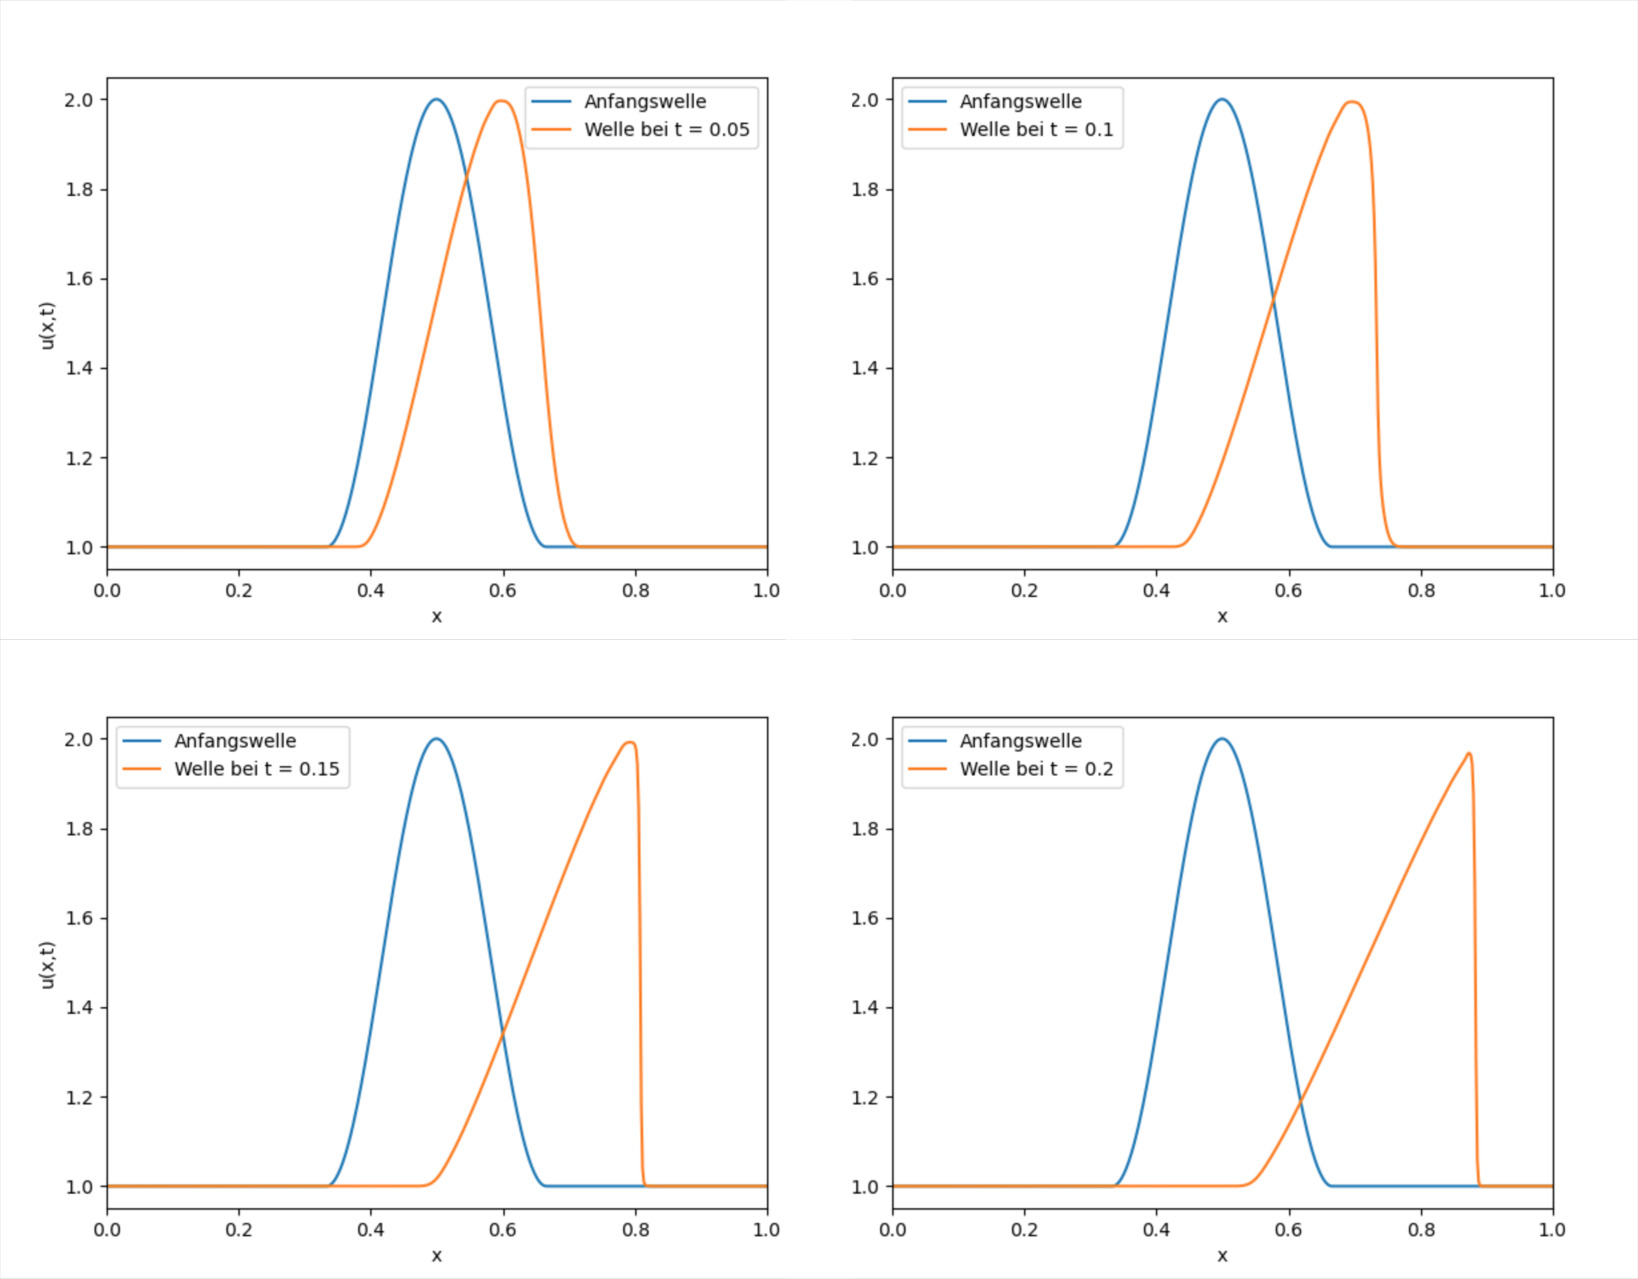
\includegraphics[width=\textwidth]{papers/luke/fig/Burger_Loesung_Welle.jpg}
	\caption{Lösung der Burgers Differenzialgleichung \eqref{luke:Burgers_DG} mit einem $sin(x)^2$ als Welle
		\label{luke:fig:Loesung_Burgers}}
\end{figure}
Abbildung \ref{luke:fig:Loesung_Burgers} zeigt die Lösung der Burgers-Gleichung mit einer nach rechts laufenden Welle, welche zu einem Überschlag der Welle führt.

Die allgemeine lineare Wellengleichung in einer Dimension lautet
\index{lineare Wellengleichung}%
\index{Wellengleichung, linear}%
\[
\partial_t^2 u - a^2 \partial_x^2 u  = 0.
\]
Dabei ist $a$ die Geschwindigkeit der Welle entlang der $x$-Achse.
Diese Wellengleichung kann in einem Bereich von $\Omega = \{(x,t)\mid t >0\}$ mit den Anfangswerten
\[
u(x,0) = u_0(x),\quad \frac{\partial u}{\partial t} = v_0(x),\quad x \in \mathbb{R},
\]
berechnet werden.
Wenn angenommen wird, dass die Geschwindigkeit $a$ konstant ist, kann die Gleichung auf die Differenzialgleichung erster Ordnung
\[
(\partial_t\mp a\partial_x)(\partial_t\pm a\partial_x) u  = 0
\]
 umgeschrieben werden.
Somit ist die Lösung der Gleichung
\begin{equation}
	\partial_t u \mp a\partial_x u = 0,
	\label{luke:Loesung_Wellengleichung}
\end{equation}
erster Ordnung automatisch eine Lösung der Wellengleichung.
Wenn nun die Gleichung \eqref{luke:Variation_loesung_2} hergenommen wird, welche über das Variationsprinzip berechnet wurde, und erneut angenommen wird, dass sich über die gesamte Zeit $t$ keine Änderung der Gesamtwassertiefe $ \nabla H = 0 $ ergibt, sowie die horizontale Koordinate $y$ konstant ist, und diese mit der Lösung der Wellengleichung \eqref{luke:Loesung_Wellengleichung} verglichen wird, dann ist zu erkennen, dass sich die Lösung über die Variation von der Lösung der Wellengleichung unterscheidet anhand dessen wie die Geschwindigkeit der Welle eingebunden ist.
Bei der Betrachtung der beiden Gleichungen
\begin{align}
	\text{Variation: }\frac{\partial \bar{u}}{\partial t} + \bar{u} \frac{\partial \bar{u}}{\partial x} = 0,
	\qquad
	\text{Wellengleichung: }\frac{\partial u}{\partial t} + a \frac{\partial u}{\partial x} = 0,
	\nonumber
\end{align}
lässt es sich leicht erkennen, dass bei der Wellengleichung die Wellengeschwindigkeit $a$ eine Konstante ist, wobei es bei der Lösung der Variation die Wellengeschwindigkeit $\bar{u}$ von der Position $x$ sowie der Zeit $t$ abhängig ist.



\printbibliography[heading=subbibliography]
\end{refsection}
